\vspace*{\subsecspace}
\section{SciSpot Design and Implementation}
\label{sec:impl}


\sysname is a general-purpose software framework for running scientific computing applications on low-cost transient cloud servers.
It incorporates policies and mechanisms for generating, deploying, orchestrating, and monitoring bags of jobs on cloud servers.
Specifically, it runs a bag of jobs defined by these parameters:
\begin{lstlisting}[basicstyle=\sffamily, frame=single, columns=fullflexible, escapeinside={(*}{*)}]
  Bag of job = {(*$\mathcal{A}$*): Application to execute,
  (*$n$*): Number of jobs,
  (*$m$*): Minimum number of jobs to finish,
  (*$\pi$*): Generator function for job parameters,
  (*$\mathcal{R}$*): Computing resources per job}
\end{lstlisting}


%Additionally, ease-of-use is one of \sysname's primary design goals, and we specifically incorporate

%it is suitable for running a large variety of applications.
\sysname seeks to minimize the cost and running time of bags of jobs of scientific computing applications.
\sysname's cost and time minimizing policies for running bags of jobs are based on empirical and analytical models of the cost and preemption dynamics of  transient cloud servers, which we present in the next section. 

\sysname is designed as a framework that increases the usability and viability of transient cloud servers for scientific computing applications, and provides a simple user interface to allow users to deploy their applications with minimum workflow changes. 
Most scientific computing applications are deployed on HPC clusters that have a batch scheduler such as Slurm~\cite{slurm} or Torque~\cite{torque}, and \sysname integrates with these schedulers (e.g., Slurm) to provide the same interface to applications. 
As shown in Figure~\ref{fig:arch},
\sysname creates and manages clusters of transient cloud servers, manages all aspects of the VM lifecycle and costs, and implements the various policies described in the rest of this section. 

\begin{figure}[t]
  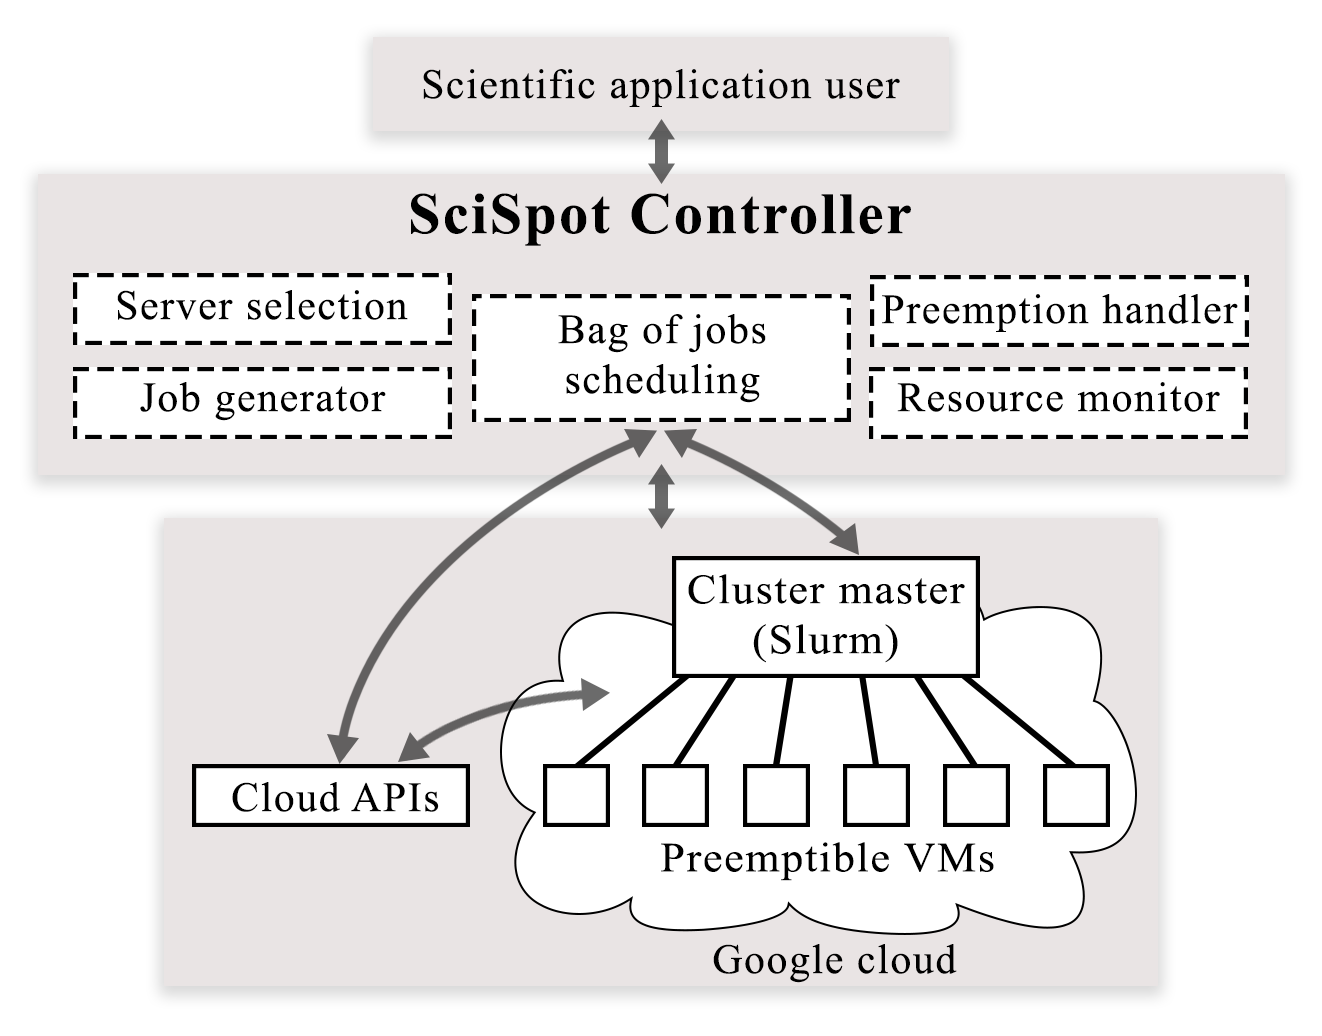
\includegraphics[width=0.3\textwidth]{../figures/Architecture.png}
\vspace*{\myfigspace}
  \caption{SciSpot architecture and system components.}
  \label{fig:arch}
  \vspace*{\myfigspace}
\end{figure}


\noindent \textbf{High-level workflow:} When a user wishes to run a bag of jobs, \sysname handles the provisioning of a cluster of transient cloud servers.
In addition, \sysname deals with the scheduling and monitoring of the bag of jobs, and with VM preemptions. 
Execution of a bag of jobs proceeds in two phases.
In the first phase, \sysname selects the ``right'' cluster configuration for a given application through a cost-minimizing exploration-based search policy, described in Section~\ref{subsec:server-selection}. 
In the second phase, \sysname proceeds to run the remaining jobs in the bag on the optimal cluster configuration. 

\prat{End design}


\sysname is implemented as a light-weight, extensible framework that makes it convenient and cheap to run scientific computing applications in the cloud.
We have implemented the \sysname prototype in Python in about 2,000 lines of code, and currently support running VMs on the Google Cloud Platform~\cite{gcp}. 
%
\sysname is implemented as a centralized controller, which implements the VM selection and job scheduling policies described in Section~\ref{sec:design}. 
The controller can run on any machine (including the user's local machine, or inside a cloud VM), and exposes an HTTP API to end-users. 
Users submit bags of jobs to the controller via the HTTP API, which then launches and maintains a cluster of cloud VMs, and maintains the job queue and metadata in a local database. 
To improve usability, we automatically generate parameter combinations for a given bag size, based on a user-provided json file with ranges and constraints for each parameter. 

\sysname integrates, and interfaces with two primary services.
First, it uses the Google cloud API~\cite{gcloud-api} for launching, terminating, and monitoring VMs.
Once a cluster is launched, it then configures a cluster manager such as Slurm~\cite{slurm} or Torque~\cite{torque}, to which it submits jobs. 
\sysname uses the Slurm cluster manager, with each VM acting as a Slurm ``cloud'' node, which allows Slurm to gracefully handle VM preemptions.
The Slurm master node runs on a small, 2 CPU non-preemptible VM, which is shared by all applications and users. 
\sysname monitors job completions and failures (due to VM preemptions) through the use of Slurm call-backs, which issue HTTP requests back to the \sysname controller.

%As part of \sysname, we also provide a base VM image with Slurm and MPI integration, along with commonly used libraries and benchmarks for scientific computing. To run an application, users must provide a location to the application source code or binaries. Integrating \sysname with container-based image management tools such as Docker~\cite{docker} and Singularity~\cite{kurtzer2017singularity} is part of our ongoing work. 





%%% Local Variables:
%%% mode: latex
%%% TeX-master: "paper"
%%% End:
